\chapter{Použité součástky}
V této kapitole budou představeny součástky, které v budoucnu použijeme.

\section{ESP32-DevkitC}
%Co to je?
ESP32-DevKitC \cite{devkitc-datasheet} je malá programovatelná deska založená na čipu ESP32\cite{ESP32} od společnosti Espressiff \cite{espressif}. Vstupní a výstupní piny se nachází na obou stranách desky, což umožňuje uživateli připojit periferní zařízení jak pomocí propojovacích vodičů, tak připojením k nepájivému poli. Na desce se také nachází mikro-USB port, který dovoluje  desku jednoduše napájet přímo z počítače, stejně jako nahrávat na desku soubory. \cite{devkitc}

\begin{figure}[htbp]
	\centering
	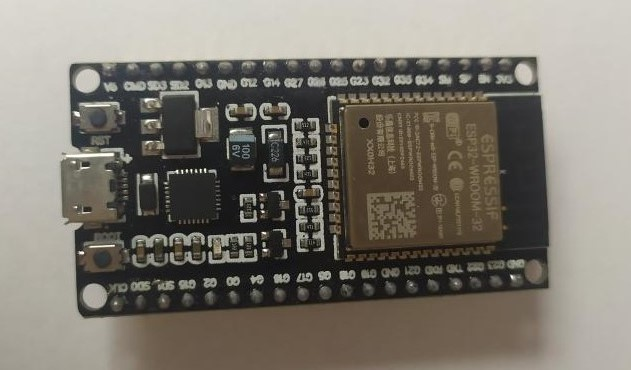
\includegraphics[width=0.5\textwidth]{img/ESPDevKit3.jpg}
	\caption{ESP32-DevKitC}
	%	\label{fig:install-sdk-3}
\end{figure}

%Co se s tím dá dělat
Deska je kompatibilní s Arduinem \cite{arduino} a často se v kombinaci zrovna s tímto typem desek používá. Díky zabudovanému Wifi modulu je možné se na součástku napojit a používat jakékoliv zařízení pracující s Wifi (například chytrý mobil), aby se k součástce napojilo a fungovalo jako dálkový ovladač. To jsem v praxi nejčastěji viděla už ke výše zmíněnému programování LED světel, ale s  ESP32-DevkitC se dá dělat prakticky cokoliv: například ho použít jako procesor pro po domácku vyrobený alarm nebo zaznamenávat počasí. 


%Proč jsem si vybrala zrovna tuto součástku.
Já se ESP32 DevkitC rozhodla použít nejen proto, že v mém okolí mělo spoustu lidí s touto technologií zkušenosti a mohli mi v případě nějakého problému jednoduše pomoct, ale hlavně kvůli dostupnosti a všestrannému využití. Navíc Wifi modul na této desce se jednoduše dá využít pro dálkové ovládání ESP32 z mobilu, což vyhovuje našim záměrům. Rozměry desky ESP32-DevkitC (přibližně 55 mm na 30 mm) jsou také vyhovující pro pozdější vybudování napájecí základny, která bude napájet a řídit LED schované v průhledné plastové květině.



\section{NeoPixel modul s 8 RGB LED WS2812}
%Co to je? Co se s tím dá dělat
Jedná se o pevný pásek s inteligentními LED za sebou. Často se využívá jako výstupní model pro Arduino a obsahuje 8 RGB LED typu WS2812,\cite {WS2812} které lze najít i pod označením NeoPixel\cite{Neopixel}. Výhoda tohoto LED pásku je, že se dá řídit pomocí jednoho datového pinu a dvou napájecích pinů, což umožňuje kontrolér ve WS diodách. Tento modul se sice nehodí našemu původnímu záměru, který vyžaduje, ale LED byly na pásku ohebném, ale jako modul pro testování postačí.

\begin{figure}[htbp]
	\centering
	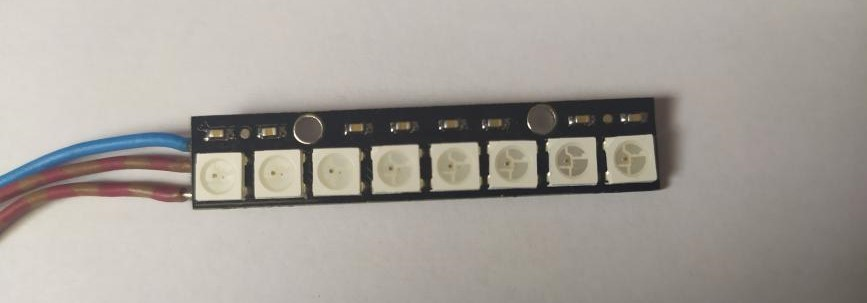
\includegraphics[width=0.5\textwidth]{img/NeoPixel2.jpg}
	\caption{RGB LED WS2812}
	%	\label{fig:install-sdk-3}
\end{figure}

%Proč jsem si vybrala zrovna tuto součástku.
Tuto součástku jsem se rozhodla použít ze dvou důvodů. Ten první byl, že jsem neměla ještě úplně jistě vybraný finální ohebný LED pásek, jaký bych chtěla použít. Druhý důvod byl stejný, jako v případě ESP32 -- kdyby nastaly při práci s tímto modulem nějaké problémy, tak jsem znala spoustu lidí, kteří by mi s případnými problémy dokázali pomoci. 

\newpage

\section{Pásek WS2812 ohebný}
Po nějaké době práce s předchozím LED páskem jsem si nakonec rozhodla vybrat skoro totožný pásek až na určitou maličkost, a to, aby byl jednoduše ohebný a tvarovatelný. Pracuje a programuje se s ním stejně, jako s předchozím páskem, avšak, jelikož to více vyhovovalo mému záměru, jsem tentokrát použila pásek se čtyřmi RGB LED.\cite{Ohebny}


\begin{figure}[htbp]
	\centering
	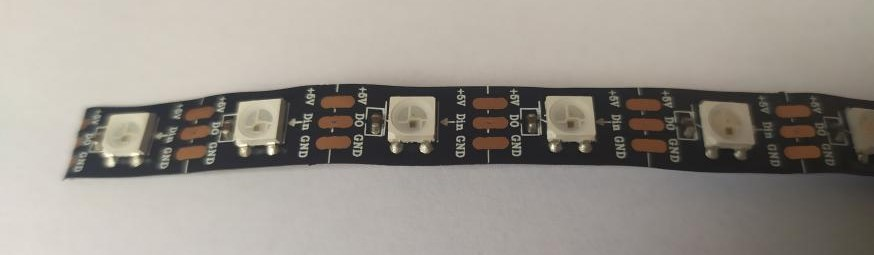
\includegraphics[width=0.5\textwidth]{img/OhebnyLedPasek2.jpg}
%<<<<<<< Updated upstream
	\caption{Pásek WS2812}
%=======
%	\caption{Pásek ws2812}
%>>>>>>> Stashed changes
	%	\label{fig:install-sdk-3}
\end{figure}


\section{Pájení}

Proto, abych s těmito součástkami mohla dál pracovat, potřebovala jsem napojit pevný LED NeoPixel pásek na ESP32-DevKitC. Což jsem udělala tak, že jsem k Neopixel pásku připájela dráty na kontakty: napájení, uzemění a vstupní pin. Na tyto dráty jsem z druhé strany přidělala pinhead a napojila jsem jej z druhé strany na ESP32-DevKitC. Jako vstupní pin jsem zvolila pin č. 21.  


%Otázky na učitele:


%Ostatní poznámky:
%Deska má tři druhy napájení, ale já budu využívat pouze napájení zkrz mikro-USB protože je to pro mě nejjednodušší. Stejně tak do toho budu posílat nahrané soubory z počítače
%Je potřeba vymyslet systém napájení
%Jak to funguje? Jaké je rozložení dané desky? 
